% !TeX program = xelatex

\documentclass{csreport}

% Document-specific settings

\graphicspath{{./images/}}

\lstloadlanguages{TeX,C++}
\lstset{defaultdialect=[LaTeX]Tex}

% Document proper

\begin{document}

% Front matter

\title{\LaTeX\ Report Template}
\subtitle{A template for reports and deliverables}
\author{Ricardo Sanz}
\date{2022/12/24}
\reference{CS-012}
\version{0.2}
\dissemination{PU - Public}
%\delno{D4.3}
%\background{myground.png}

\maketitle

\executivesummary

This document is an example of use with some basic explanations of the \LaTeX\ class \texttt{csreport.cls}. This class is to be used in CORESENSE large reports, esp. deliverables.

We acknowledge the financial support through the contract \#101070254, \emph{CoreSense: A Hybrid Cognitive Architecture for Deep Understanding} granted by the European Commission inside the Horizon Europe programme.
 

\documentversions
\versionitem{0.0}{Initial draft}{R.Sanz}{2022/06/20}
\versionitem{0.1}{Cover reformatting}{R.Sanz}{2022/11/03}
\versionitem{0.2}{Adaptation to color schema}{R.Sanz}{2022/12/24}

\tableofcontents



% Main matter

%%%%%%%%%%%%%%%%%%%%%%%%%%%%%%%%%%%%%%%%%%%%%%%%%%%%%%%%%%%%%%%%%%%%%%%%%%%%

\chapter{Introduction}

This brief report describes the \textbf{CORESENSE template for reports and deliverables}. It is a template based on the \LaTeX\ document processing system \cite{Lamport-1986}.

The default formatting of a \LaTeX\ document is determined by the \emph{class} used by that document at the very begining of the source file. 

This document describes the CORESENSE \LaTeX\ template for reports and deliverables that is provided in the form of a class file: \code|csreport.cls| and additional resource files that will be described below.

The logos, colors and fonts of this template are based on the CORESENSE Brand Guidelines \cite{CORESENSE-017}.

\vfill

\quotecite{Precisely how much of the business of thinking a machine
could possibly be made to perform, and what part of it must be left
for the living mind, is a question not without conceivable practical
importance; the study of it can at any rate not fail to throw
needed light on the nature of the reasoning process.}{Peirce-1887}

%%%%%%%%%%%%%%%%%%%%%%%%%%%%%%%%%%%%%%%%%%%%%%%%%%%%%%%%%%%%%%%%%%%%%%%%%%%%

\chapter{The CSreport \LaTeX\ template}

%===========================================================================
\section{Template description}

The \code|csreport.cls| class file is based on the basic \code|report.cls| class of \LaTeX. It redefines some of the macros and defines new ones to create a homogeneous style for CORESENSE internal documentation. 

This is how a document formatted with this template looks like:

\begin{center}
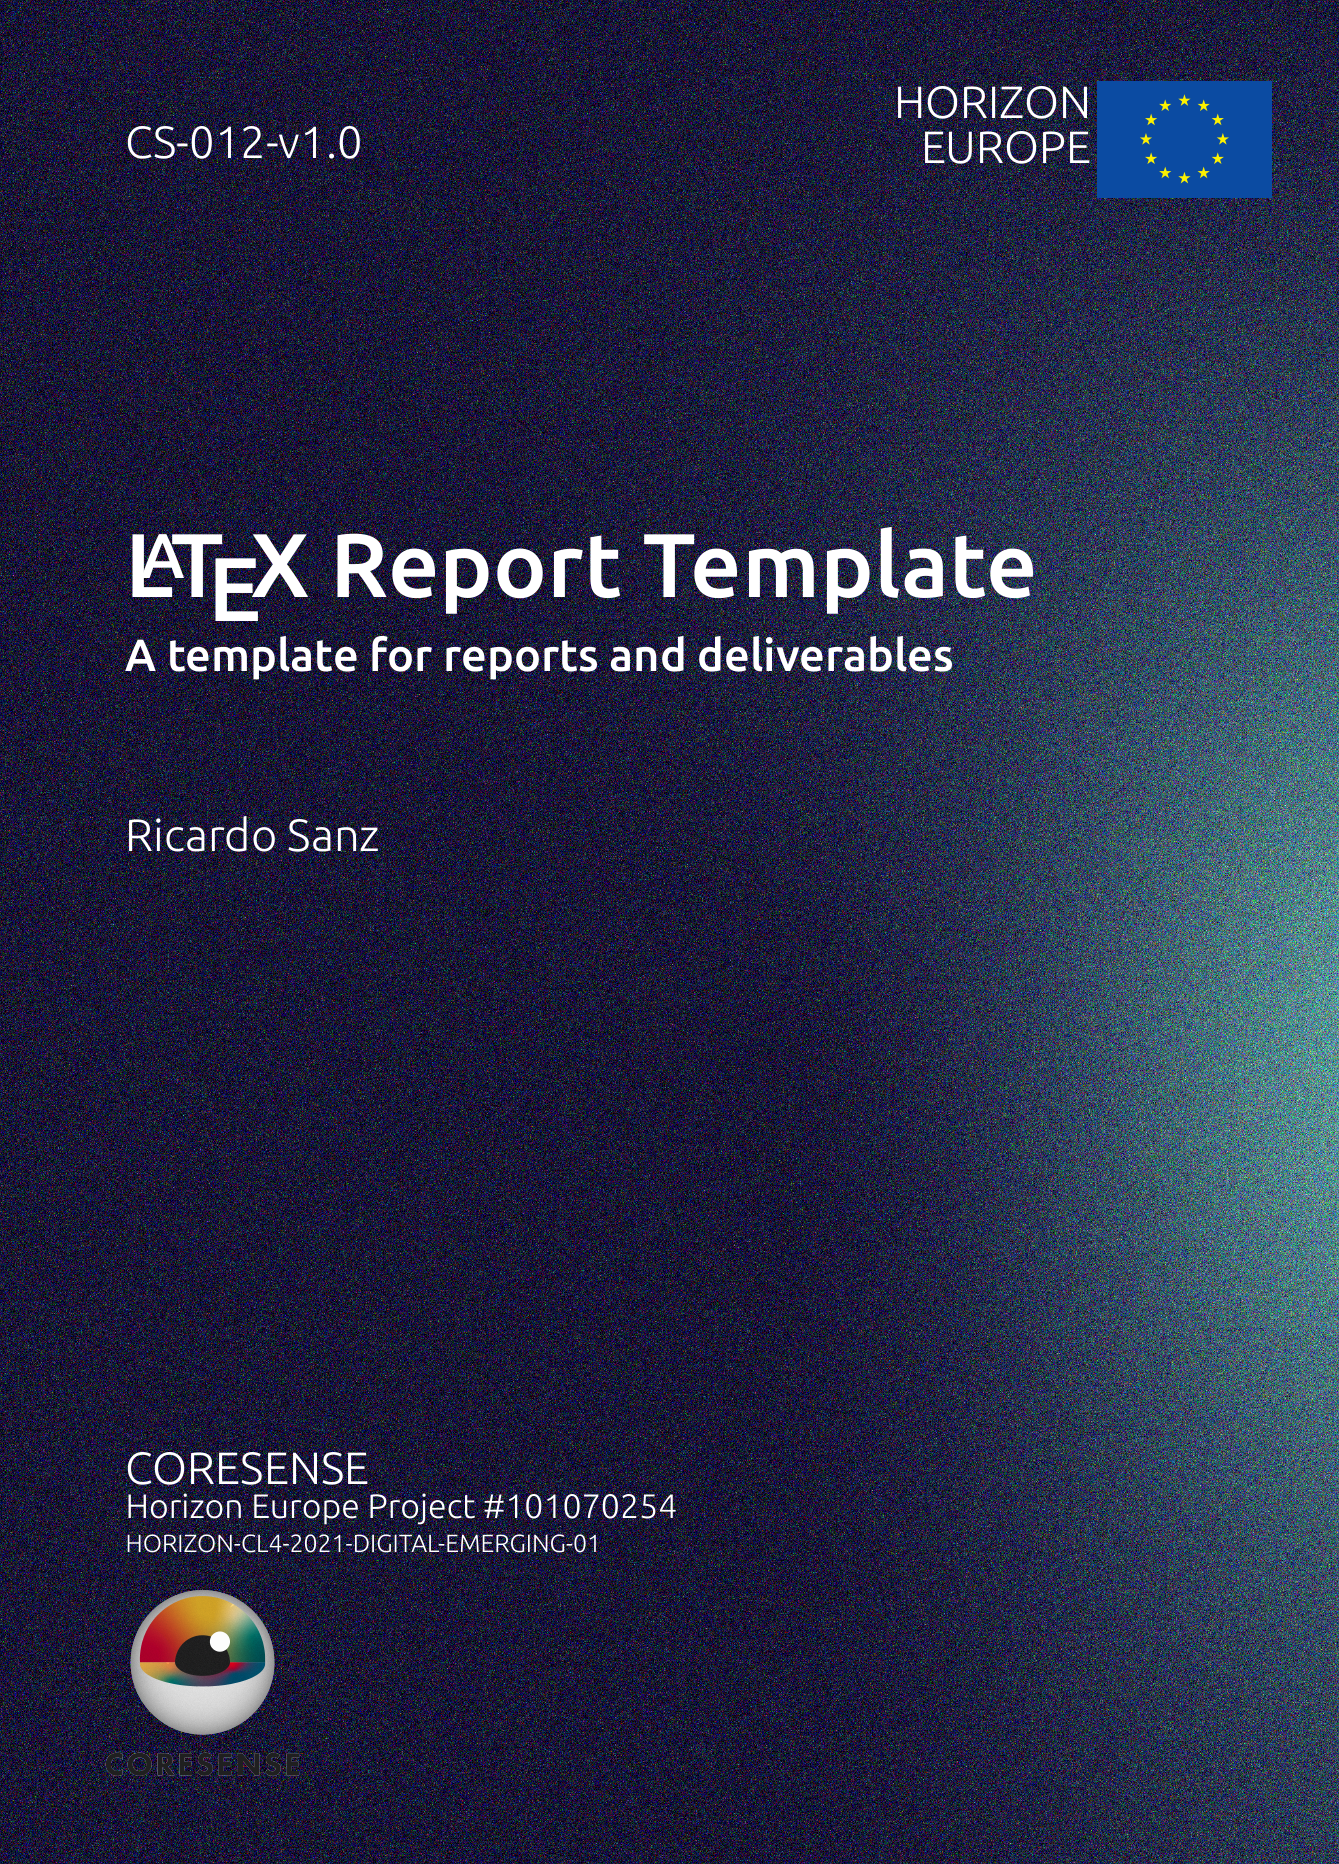
\includegraphics[height=10cm,frame]{csreportcover.png}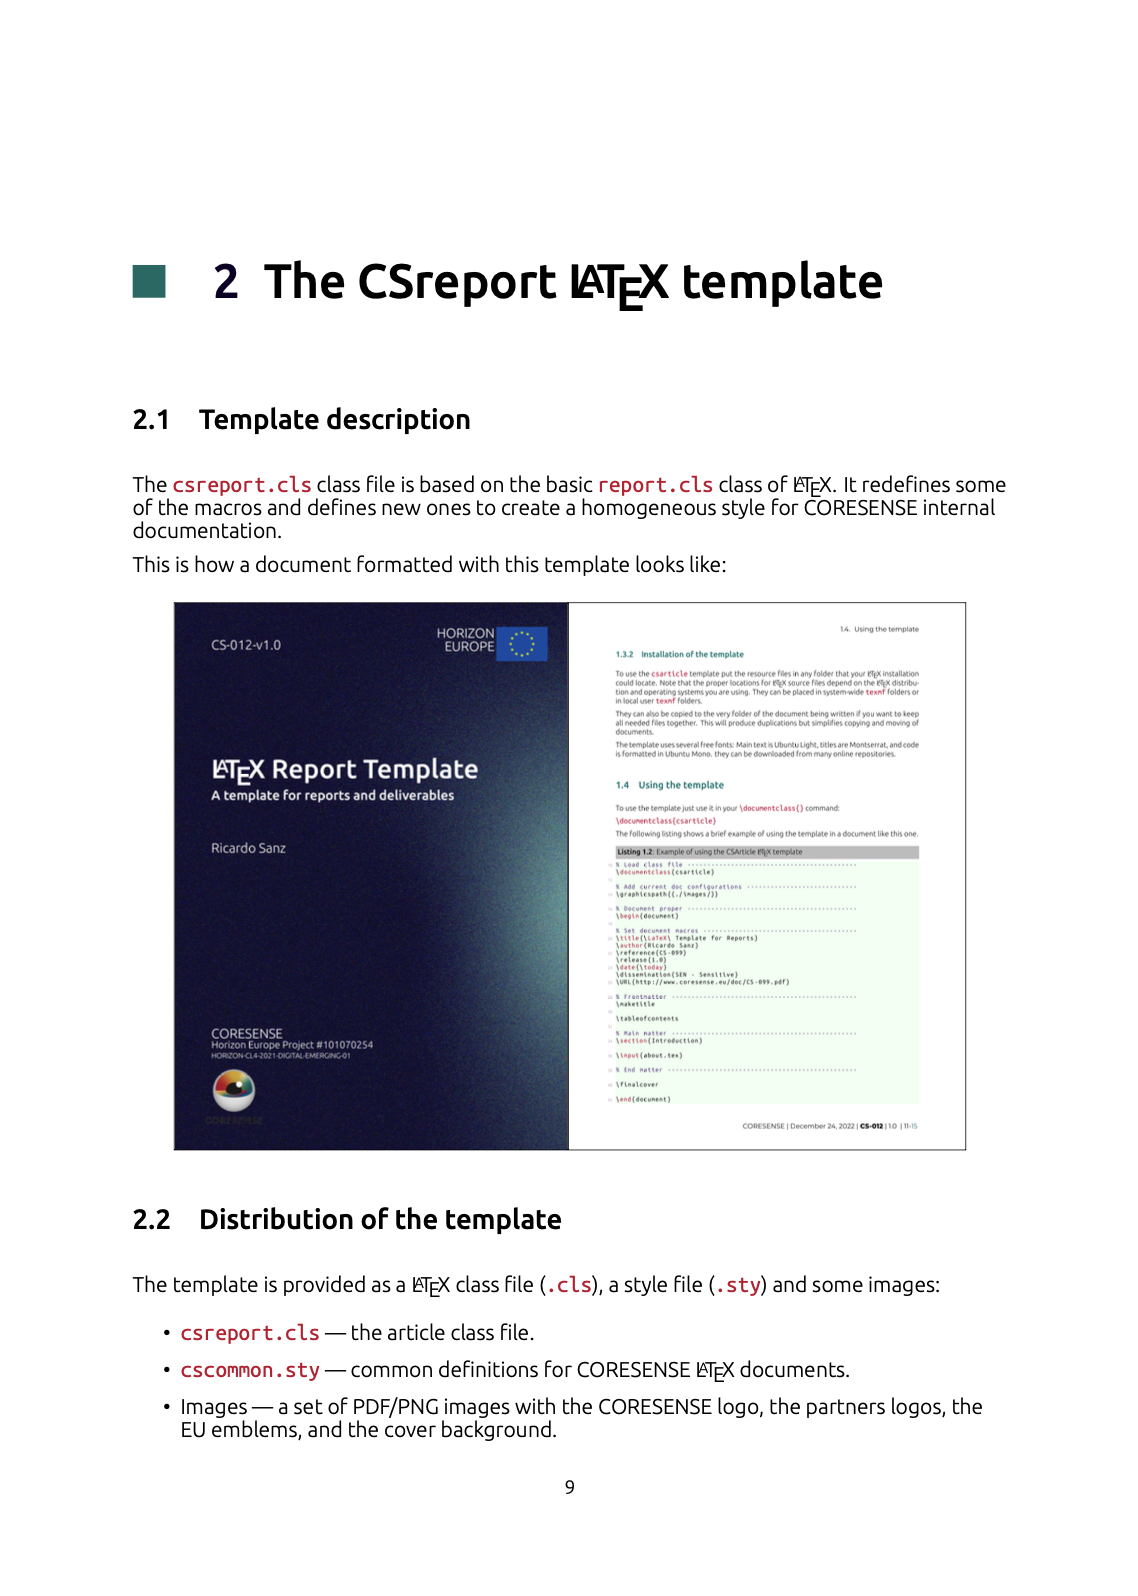
\includegraphics[height=10cm,frame]{csreportpage.png}
\end{center}

\section{Distribution of the template}

The template is provided as a \LaTeX\ class file (\code|.cls|), a style file (\code|.sty|) and some images:

\begin{itemize}
\item \code|csreport.cls| --- the article class file. 
\item \code|cscommon.sty| --- common definitions for CORESENSE \LaTeX\ documents.
\item Images --- a set of PDF/PNG images with the CORESENSE logo, the partners logos, the EU emblems, cover background, etc.
\end{itemize}

The source file used to generate this document (\code|csreport.tex|) is also distributed with the template as an example of use.  

The template uses the following fonts: \code|Ubuntu Light| for main text body; \code|Montserrat| for titles\footnote{Google Montserrat is similar to Adobe Futura but can be used freely.}; and \code|Ubuntu Mono| for code. 

\section{Installation of the template}

To use the \code|csreport| template put the resource files in any folder that your \LaTeX\ installation could locate. Note that the proper locations for \LaTeX\ source files depend on the \LaTeX\ distribution and operating systems you are using. They can be placed in system-wide \code|texmf| folders or in local user \code|texmf| folders. 

They can also be copied to the very folder of the document being written if you want to keep all needed files together. This will produce duplications but simplifies copying and moving of documents.

The template uses several free fonts: Main text is Ubuntu Light, titles are Montserrat, and code is formatted in Ubuntu Mono. they can be downloaded from online free repositories.

\section{Template Packages}

The template class file pre-uploads the following packages:

\begin{table}[h!]
\centering
\renewcommand{\arraystretch}{1.2}
\caption{Pre-uploaded Packages}\label{tab:packages}
\begin{tabular}{|c|c|}\hline 
\tabtitle{Package} & \tabtitle{Use for} \\    \hline \hline
\bko listings & to include code listings (see \LaTeX\ example above)\\ \hline
\bko titlesec & to change section titles format\\ \hline
\bko hyperref & to handle hypereferences\\ \hline
\bko fontspec & \bkx to change document font\\ \hline
\bko graphicx & to include graphics\\ \hline
\bko tikz & \bkm to create graphics (e.g. generate the EU flag).\\ \hline
\end{tabular}
\renewcommand{\arraystretch}{1}
\end{table}

\section{Template Colors}

The template defines the colors that are shown in Table \ref{tab:colors}. You can use any color using the \code|\color{}| command; e.g.:

\begin{verbatim}
{\color{CSGray}This text is CORESENSE gray and this one is 
 \color{CSOrange} CORESENSE yellow.}
\end{verbatim}

renders this:

{\color{CSGray}This text is CORESENSE gray and \color{CSOrange} this one is CORESENSE yellow.} 

\begin{table}\centering
\caption{Template colors (name, RGB, example).}
\label{tab:colors}
\renewcommand{\arraystretch}{0.4}
\begin{tabular}[h!]{|l|l|l|}\hline
\tabtitle{Name} & \tabtitle{HTML} & \tabtitle{Color} \\ \hline \hline
\bko CSGreen & HTML(\#006A63) & \color{CSGreen}\rule{1cm}{1cm}\color{white}\rule{0cm}{1.07cm}\\\hline
\bkl CSRed & HTML(\#BF002A) & \color{CSRed}\rule{1cm}{1cm}\color{white}\rule{0cm}{1.07cm}  \\\hline
\bko CSRussianGray & HTML(\#0C0026) & \color{CSRussianGray}\rule{1cm}{1cm}\color{white}\rule{0cm}{1.07cm} \\\hline
\bkl CSMaroon & HTML(\#512977) & \color{CSMaroon}\rule{1cm}{1cm}\color{white}\rule{0cm}{1.07cm} \\\hline
\bko CSOrange & HTML(\#EAB82D) & \color{CSOrange}\rule{1cm}{1cm}\color{white}\rule{0cm}{1.07cm}\\\hline
\bkl CSLightGreen & HTML(\#009990) & \color{CSLightGreen}\rule{1cm}{1cm}\color{white}\rule{0cm}{1.07cm}\\\hline
\bko CSUltraLightGreen & HTML(\#EEFFF0) & \color{CSUltraLightGreen}\rule{1cm}{1cm}\color{white}\rule{0cm}{1.07cm}\\\hline
\bkl CSLightOrange & HTML(\#FAD85D) & \color{CSLightOrange}\rule{1cm}{1cm}\color{white}\rule{0cm}{1.07cm}\\\hline
\bko CSUltraLightOrange & HTML(\#FFE499) & \color{CSUltraLightOrange}\rule{1cm}{1cm}\color{white}\rule{0cm}{1.07cm}\\\hline
\bkl CSLightMaroon & HTML(\#613997) & \color{CSLightMaroon}\rule{1cm}{1cm}\color{white}\rule{0cm}{1.07cm}\\\hline
\bko CSUltraLightMaroon & HTML(\#B1A9f7) & \color{CSUltraLightMaroon}\rule{1cm}{1cm}\color{white}\rule{0cm}{1.07cm}\\\hline
\bkl CSGray & HTML(888888) & \color{CSGray}\rule{1cm}{1cm}\color{white}\rule{0cm}{1.07cm} \\  \hline
\bko CSLightGray & HTML(BBBBBB) & \color{CSLightGray}\rule{1cm}{1cm}\color{white}\rule{0cm}{1.07cm} \\  \hline
\bkl CSUltraLightGray & HTML(EEEEEE) & \color{CSUltraLightGray}\rule{1cm}{1cm}\color{white}\rule{0cm}{1.07cm} \\  
\hline
\end{tabular}
\renewcommand{\arraystretch}{1}
\end{table}


%%%%%%%%%%%%%%%%%%%%%%%%%%%%%%%%%%%%%%%%%%%%%%%%%%%%%%%%%%%%%%%%%%%%%%%%%%%%%%%%%%%%%%%%%%%

\chapter{Using the template}

\section{Creating a report}

The formatting of a \LaTeX\ document is determined by the \emph{class} used by that document at the very begining of the source file: 

\code|\documentclass{article}|

The default look can then be changed by means of including extra \emph{packages} or redefining some of the commands or parameters. 

\code|\usepackage{fancyhdr}|

The class file names have the \code|.cls| extension, the package file names have the \code|.sty| extension. 

\begin{lstlisting}[language=TeX,caption={Example of using the CSReport \LaTeX\ template}]
% Load class file -------------------------------------------
\documentclass[a4paper,11pt]{csreport}

% Add current doc configurations ----------------------------
\graphicspath{{./images/}}

% Document proper -------------------------------------------
\begin{document}

% Set document macros ---------------------------------------
\title{CoreSense Report Template}
\subtitle{A \LaTeX\ template}
\author{Ricardo Sanz}
\copyrightyear{2022}
\reference{CS-R-XXX}
\release{0.0}
\status{Draft}
\dissemination{SEN - Sensitive}

% Frontmatter -----------------------------------------------
\maketitle

\documentversions
\versionitem{0.0}{Initial draft}{R.Sanz}{2022/06/20}

\tableofcontents

% Main matter -----------------------------------------------
\chapter{Introduction}
\input{about.tex}

% End matter ------------------------------------------------
\finalcover

\end{document}
\end{lstlisting}


\section{Template Macros}

These are the macros provided by the template; some of them are the same as the base \code|report| class:

\begin{description}
\item[\textbackslash title\{\}] --- Sets the title of the document.
\item[\textbackslash author\{\}] --- Name of author.
\item[\textbackslash date\{\}] --- Date of the document.
\item[\textbackslash reference\{\}] --- Reference (See CORESENSE controlled documents list).
\item[\textbackslash release\{\}] --- Release (See CORESENSE controlled documents list).
\item[\textbackslash URL\{\}] --- Link to download the document.
\item[\textbackslash delno\{\}] --- Specify a number for a deliverable.
\item[\textbackslash background\{\}] --- Select background image for cover.
\item[\textbackslash approval\{\}] --- Approval signatures for deliverables.
\item[\textbackslash documentversions\{\}] --- Start versions page.
\item[\textbackslash versionitem\{\}] --- Add version item.
\item[\textbackslash URL\{\}] --- Link to download the document.
\item[\textbackslash finalcover] --- Generate final cover with data, acknowledgements and disclaimer.
\item[\textbackslash euflag\{\}] --- Generate an EU flag; e.g. \code|\euflag{0.02}| generates this \euflag{0.02}.
\item[\textbackslash code\{\}] --- Change font to monospaced colored (to highlight code).
\item[\textbackslash tabtitle\{\}] --- Change table title to green background. See Table \ref{tab:packages} below for an example.
\item[\textbackslash bkg,bkr,bkl,bkma,bko,bkx] --- Change table cell background to green, red, light green, ligh maroon, light orange, and light gray.
\item[\textbackslash quotecite\{\}\{\}] --- Insert a quotation with a cite to bibliography.
\end{description}


Example of use of the \code|\quotecite{...}{Sowa-2007}}|:

\quotecite{A procedure is used in only one way, but a declarative specification can be used in many different ways.}{Sowa-2007}


Example of use of the macros for coloring tables:

\begin{lstlisting}[language=TeX,caption={\LaTeX\ code for Table \ref{tab:packages}}]
\begin{table}[h!]
\centering
\renewcommand{\arraystretch}{1.2}
\caption{Pre-uploaded Packages}\label{tab:packages}
\begin{tabular}{|c|c|}\hline 
\tabtitle{Package} & \tabtitle{Use for} \\    \hline \hline
\bko listings & to include code listings (see \LaTeX\ example above)\\ \hline
\bko titlesec & to change section titles format\\ \hline
\bko hyperref & to handle hypereferences\\ \hline
\bko fontspec & \bkx to change document font\\ \hline
\bko graphicx & to include graphics\\ \hline
\bko tikz & \bkm to create graphics (e.g. generate the EU flag).\\ \hline
\end{tabular}
\renewcommand{\arraystretch}{1}
\end{table}
\end{lstlisting}


\section{\TeX\ Engine}

This template uses the \code|fontspec| package and shall be compiled with \code|xelatex|.



%%%%%%%%%%%%%%%%%%%%%%%%%%%%%%%%%%%%%%%%%%%%%%%%%%%%%%%%%%%%%%%%%%%%%%%%%%%%%%%%%%%%%%%%%

\section{Using the template for deliverables}

In case of using this template for project formal deliverables, please follow these rules:

\begin{enumerate}
\item Set the deliverable number (e.g. \code|D4.3|) using the command \code|\delno{D4.3}| and the deliverable name as as \code|\title{Report on Experimental Understanding}|.
\item Use \code|\subtitle{}| to make any precision or highlight some aspect of particular relevance. You may also leave it empty.
\item Identify the partner organisation in the authors list (e.g. \code|\author{R.Sanz (UPM)}|).
\item Establish the dissemination level of the deliverable with \code|\dissemination{}|. Our dissemination levels are only two: PU - Public and SEN - Sensitive.
\item Verify that the list of document versions is complete and correct.
\item Add a \code|\approval{}| section after the list of versions (when the deliverable is approved by WPL, PM, and QA).  
\end{enumerate}


For example, the following code for the approval:

\begin{lstlisting}[language=TeX,caption={\LaTeX\ code for Table \ref{tab:packages}}]
\approval{N.Hammoudeh (FHG)}{2022/12/13}
         {R.Sanz (UPM)}{2022/12/14}
         {C.García (IMR)}{2022/12/14}
\end{lstlisting}

Will render this into the document at the bottom of the page where it appears:

\begin{minipage}{12cm}
\approval{N.Hammoudeh (FHG)}{2022/12/13}
         {R.Sanz (UPM)}{2022/12/14}
         {C.García (IMR)}{2022/12/14}
\end{minipage}

The cover of a deliverable contains some more information than a conventional report. This is how the deliverable cover is rendered:

\begin{center}
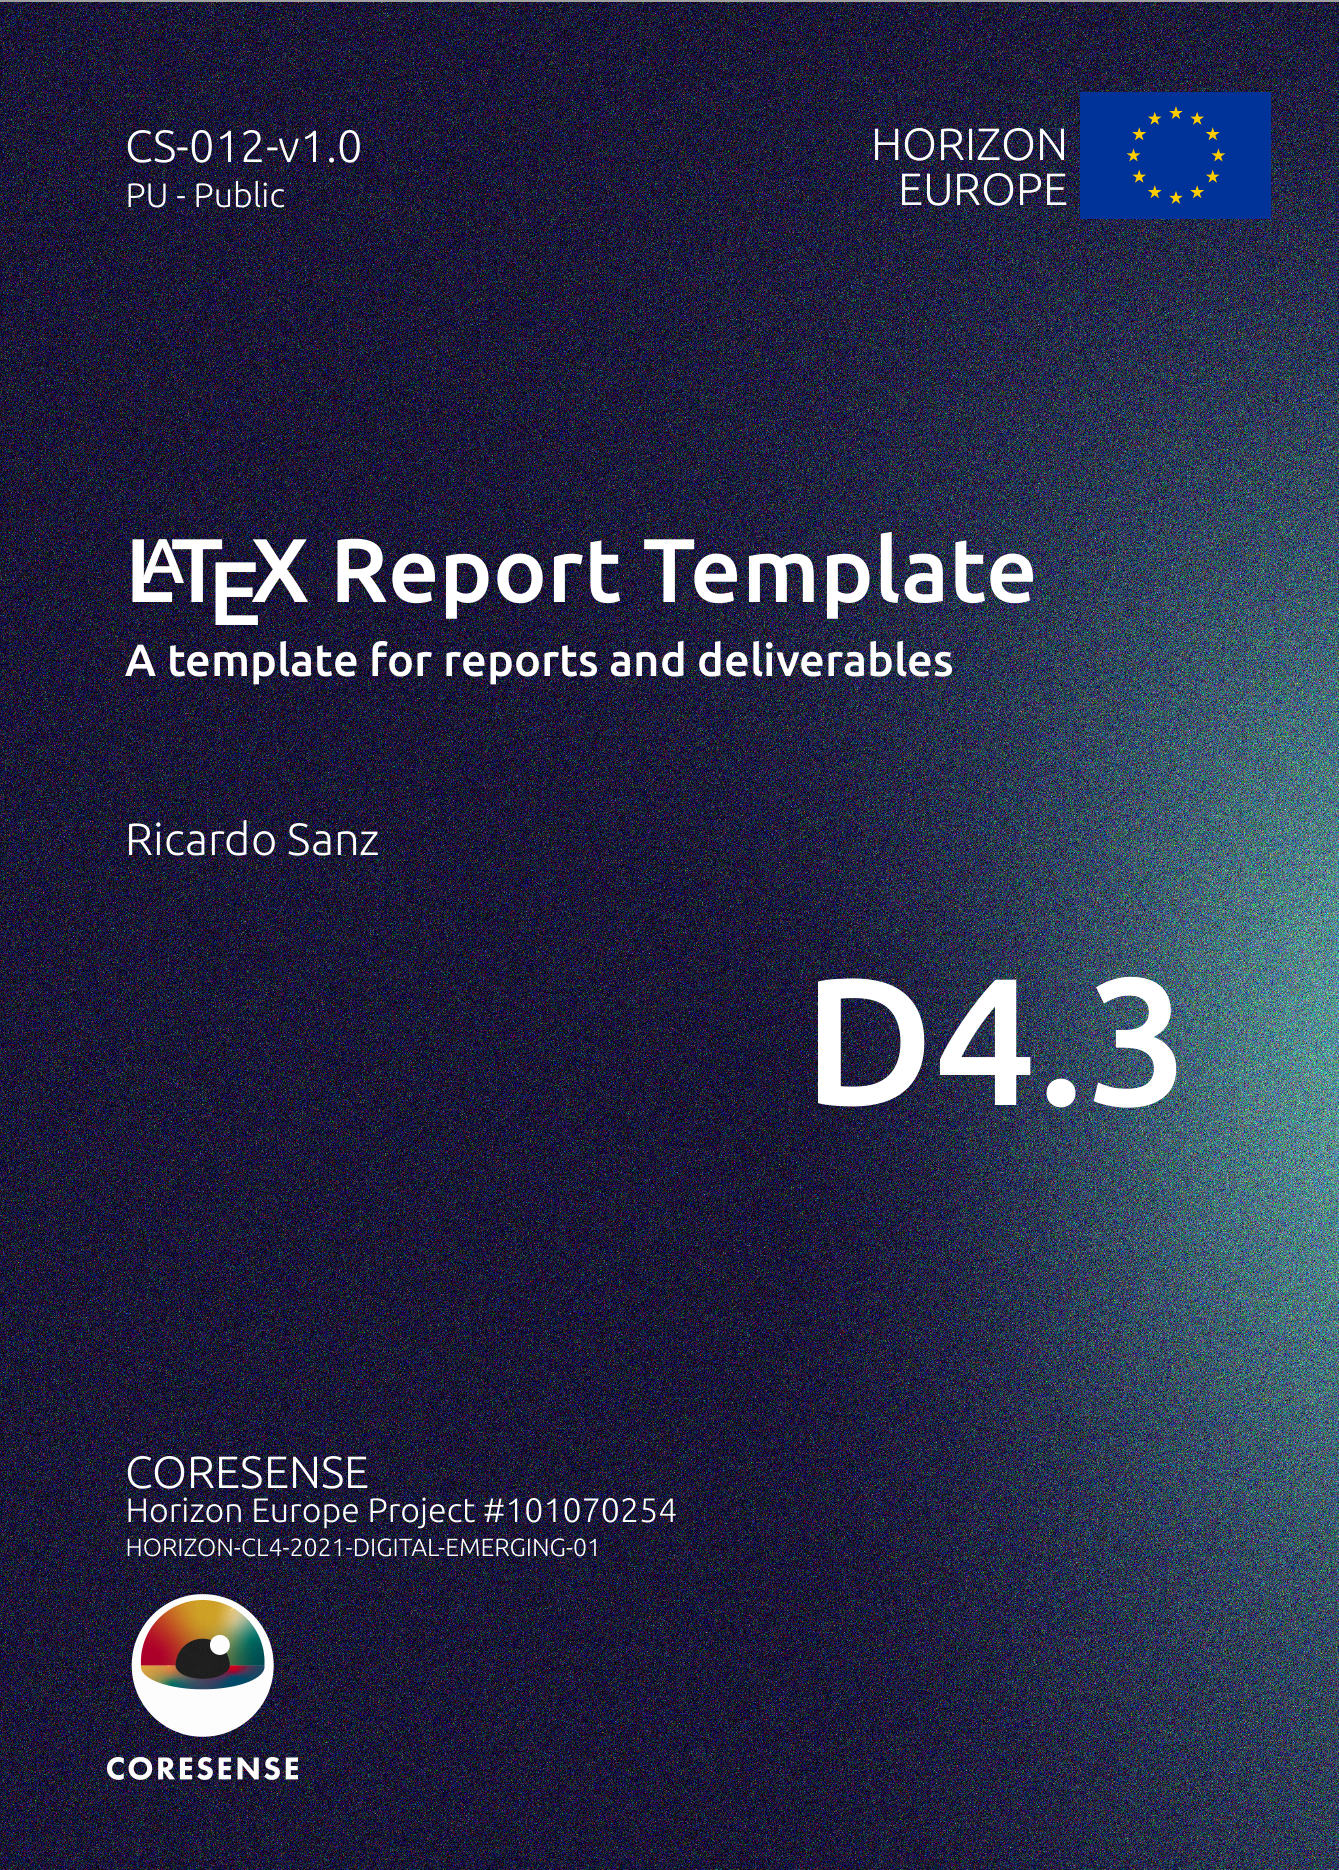
\includegraphics[height=10cm,frame]{csdeliverablecover.png}
\end{center}


% Back matter ===================================================================

\bibliography{library}
\bibliographystyle{apalike}

\finalcover

\end{document}


